\section{Fachliche Konzeption}

\descriptionWhat{Vollständige Umsetzungsbeschreibung der konkreten Lösung}

\subsection{z.B. Ziel- Nutzergruppe}
\descriptionWhat{Zielgruppendefinition}

Primäre Zielgruppen sind die Technologiestiftung Berlin (TSB) und der Verein Flussbad Berlin (VFB). Des weiteren sind die erhobenen Daten für Dritte zugänglich und relevant. Die TSB ist als Auftraggeber von besonderer Bedeutung\rem{, das fertige Produkt muss ihren Anforderungen entsprechen}. Der VFB ist als Partner für die Messstandorte besonders für die Erprobungsphase wichtig. Der Prototyp muss eventuell auch an die Gegebenheiten des vom VFB zur Verfügung gestellten Standortes angepasst werden.

\subsection{z.B. Inhaltlicher Aufbau/Komponenten}

\descriptionWhat{Dokumentenstruktur, Web-Seitenstruktur, Seitenstruktur Bauteile, Konstruktionspläne}

\subsubsection{Messstation}
Die Messstation besteht aus einem Arduino Uno als basisplatform (siehe~\autoref{fig:ardoinoUno}). Einem Dragino-Shiled für die Kommunikation mittels des LoRaWAN Protokoll (siehe~\autoref{fig:draginoShield}). Für die Erfassung der Wasserdaten kommen Sensoren für pH-Wert, Trübheit sowie Temperatur zum Einsatz. Der Arduino und das Dragino-Shiled sind in einem Wetterfesten Gehäuse untergebracht. Das Gehäuse hat mindestens die Schutzklasse IP65 damit die Komponenten ausreichend gegen nässe geschützt sind. Die Sensoren sind außerhalb des Gehäuses und durch Wasserfeste Kabeldurchführungen verbunden. Die Energieversorgung der Messstation wird über eine externe Stromversorgung sichergestellt.

\begin{figure}[H]
	\centering
	\begin{minipage}[t]{0.45\linewidth}
		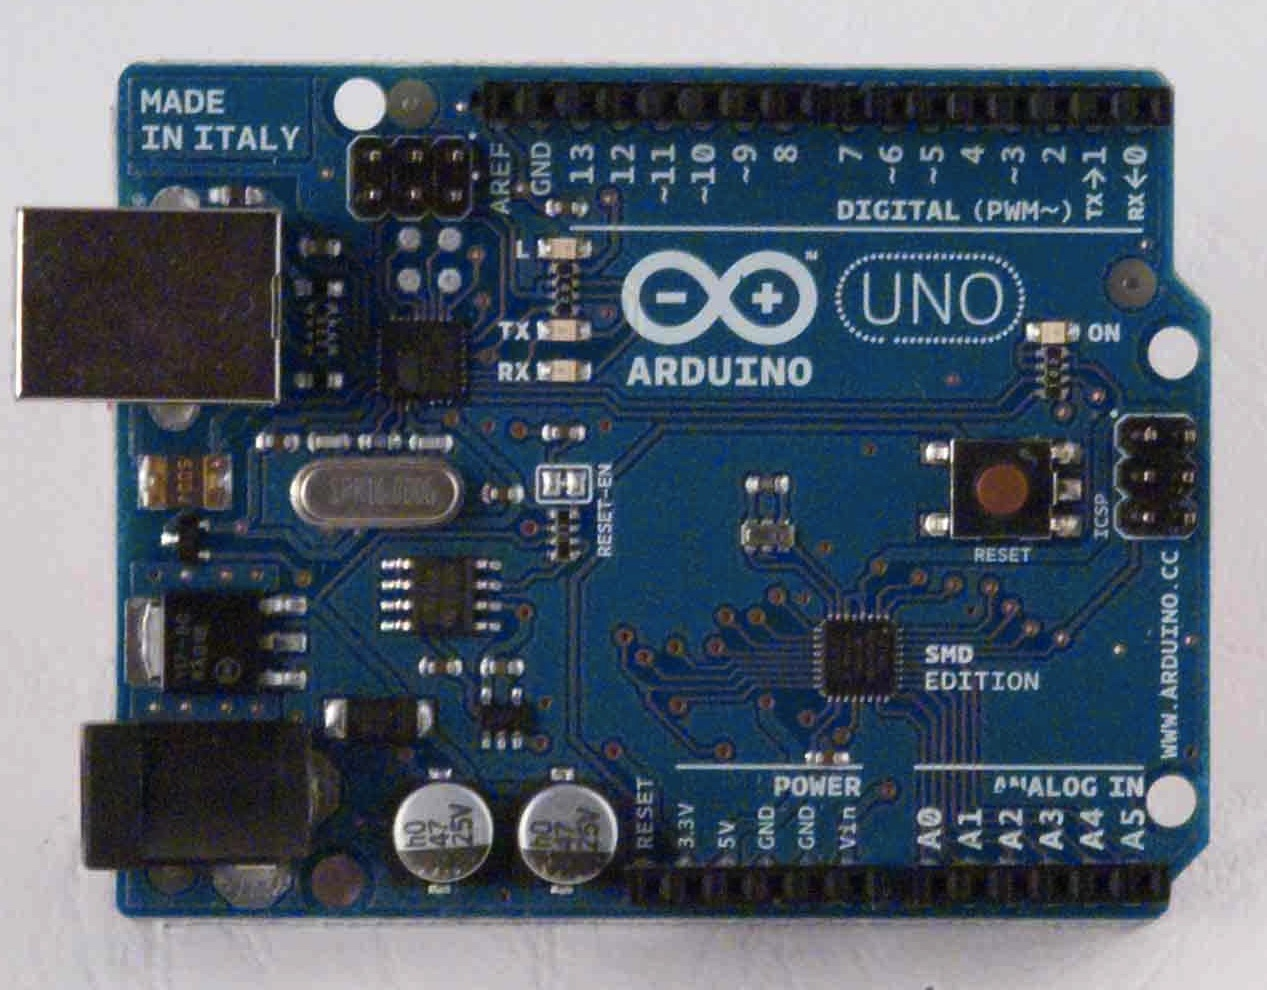
\includegraphics[width=7cm]{figures/ArduinoUnoSMDFront.jpg}
		\caption{Arduino Uno der SMD Variante. Veröffentlicht auf \href{https://www.arduino.cc/en/Main/ArduinoBoardUnoSMD}{Arduino.cc}}
		\label{fig:ardoinoUno}
	\end{minipage}
	\hfill
	\begin{minipage}[t]{0.45\linewidth}
		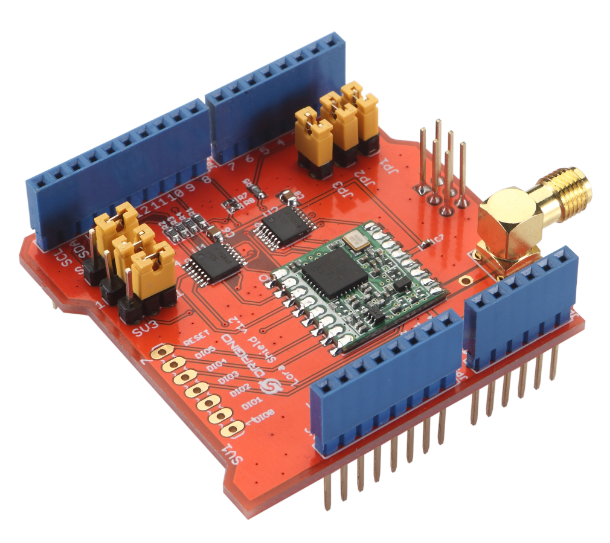
\includegraphics[width=7cm]{figures/LoraShield-1.png}
		\caption{Dragino LoRa Shield. Veröffentlicht auf \href{http://www.dragino.com/products/lora/item/102-lora-shield.html}{dragino.com}}
		\label{fig:draginoShield}
	\end{minipage}
\end{figure}

\subsubsection{Datenbankserver}
Für das speichern der empfangenen Daten kommt ein MySQL Datenbanksystem zum Einsatz. Hier werden sämtliche vom TTN übermittelten Daten abgelegt. Die Daten werden nicht im Rohformat gespeichert. Nach Auswertung des JSON Strings sind die Werte nach Metadaten, Messwert und Node in der Datenbank abgelegt.

\subsubsection{Datenmodell}
\begin{figure}[H]
	\centering
	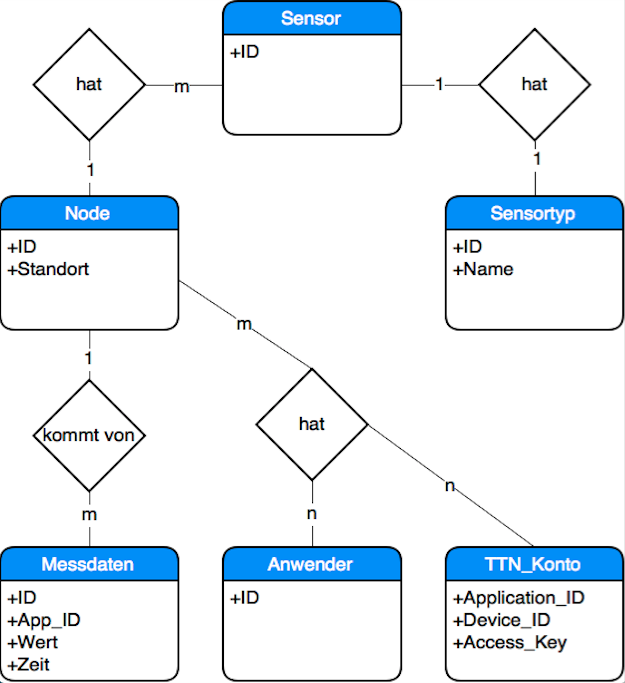
\includegraphics[width=6cm]{figures/dbmodel.png}
	\caption{Datenbankmodel}
	\label{fig:dbModel}
\end{figure}

\subsubsection{Webserver}
Der Webserver hat folgende Funktionalität:
\begin{itemize}
	\item Eine Schnittstelle für TTN um die Daten von dort zu empfangen. Die Daten werden im JSON Format übertragen. Bei Empfang werden diese dann in der Datenbank gespeichert. Da es sich um eine URL basierte schnittstelle handelt werden nur POST-request's verarbeitet. So wird verhindert das ein URL aufruf mittels eines Browsers fremddaten hinzufühgt.
	\item Eine Schnittstelle die zum Abrufen der gespeicherten Daten. Die Daten werden mittels eines GET-request und Parametern in der Abfrage bereitgestellt. Ein einfaches Web-Formular dient als Generator zum erstellen der URL.
\end{itemize}
Desweiteren dient der Webserver zur präsentation des Projektes.

\subsubsection{Use Case}
\begin{figure}[H]
	\centering
	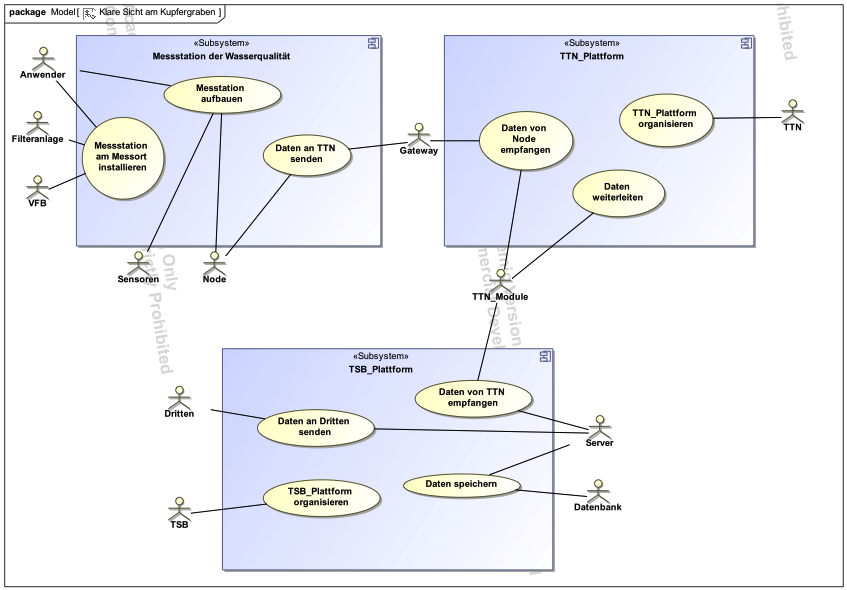
\includegraphics[width=10cm]{figures/use-case.png}
	\caption{Use-Case model}
	\label{fig:useCase}
\end{figure}